\documentclass[tikz,border=2pt]{standalone}
\usepackage{amsmath,amssymb}
\usepackage{pgfplots}
\pgfplotsset{compat=1.18}
\usetikzlibrary{arrows.meta}

\begin{document}
% f(x) = x, g(x) = x^2, h(x) = 2x^2 + x near 0: g(x)/f(x) = x -> 0 and g(x)/h(x) = x/(2x+1) -> 0,
% so g = o(f) and g = o(h) as x -> 0.
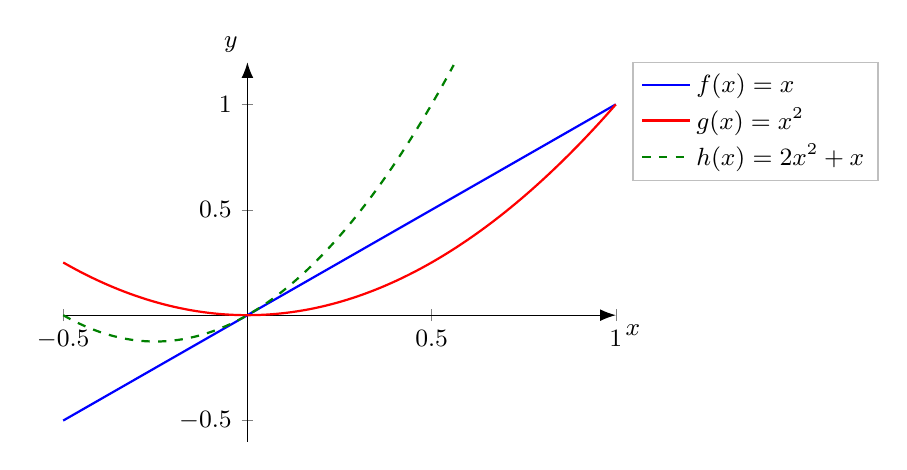
\begin{tikzpicture}[every node/.style={font=\small}]
	\begin{axis}[
		width=8.6cm, height=6.4cm,
		axis lines=middle, axis line style={-{Latex[length=2mm]}},
		xmin=-0.5, xmax=1, ymin=-0.6, ymax=1.2,
		xtick={-0.5,0.5,1}, ytick={-0.5,0.5,1},
		tick label style={font=\small},
		xlabel={$x$}, ylabel={$y$},
		xlabel style={below right}, ylabel style={above left},
		legend pos=outer north east, legend cell align={left},
		legend style={font=\small, draw=gray!50, fill=white},
		samples=100, clip=false
		]
		\addplot[blue, thick, domain=-0.5:1] {x};
		\addlegendentry{$f(x)=x$}
		\addplot[red, thick, domain=-0.5:1] {x^2};
		\addlegendentry{$g(x)=x^2$}
		\addplot[green!50!black, thick, dashed, domain=-0.5:0.56] {2*x^2+x};
		\addlegendentry{$h(x)=2x^2+x$}
	\end{axis}
\end{tikzpicture}
\end{document}
